\chapter{绪论}
\label{cha:intro}

\section{研究背景与研究意义}
\label{sec:chap1:backgroud}
航空航天及空间卫星技术是新时代高新科技的典型代表,越来越多的国家加入到研制、发射航天器的行列,人类已经进入了“太空时代”。美国前总统肯尼迪曾预言:“谁控制了宇宙,谁就控制了地球;谁控制了空间,谁就控制了战争的主动权。”世界各国在竞争与博弈中都在进行太空探索,以充分利用太空领域的军事及经济资源。中国航空航天技术及其相关产业经过~60~年的发展,已经取得了以“两弹一星”、载人航天、月球探测为代表的辉煌成就。

作为航空航天及空间卫星上的关键技术~\raisebox{0.5mm} {------}~空间电源系统,其技术水平及可靠程度直接影响到整个航空航天卫星工作的稳定性。太空宇航任务对空间电源系统的稳定性要求日益提高,必须保证在所设计的整个生命周期内提供稳定可靠的供电性能,满足航空航天卫星的工作需求。目前航空航天卫星多为遥感卫星,载荷系统中以感性、容性负载居多,在供电时对电源系统有较大的冲击。此外,SAR~航天卫星电源系统广泛采用的多母线架构增加了电源系统结构的复杂程度,相比于传统的卫星电源系统,更难保证稳定性及可靠性。
\begin{figure}[h]
  \centering
     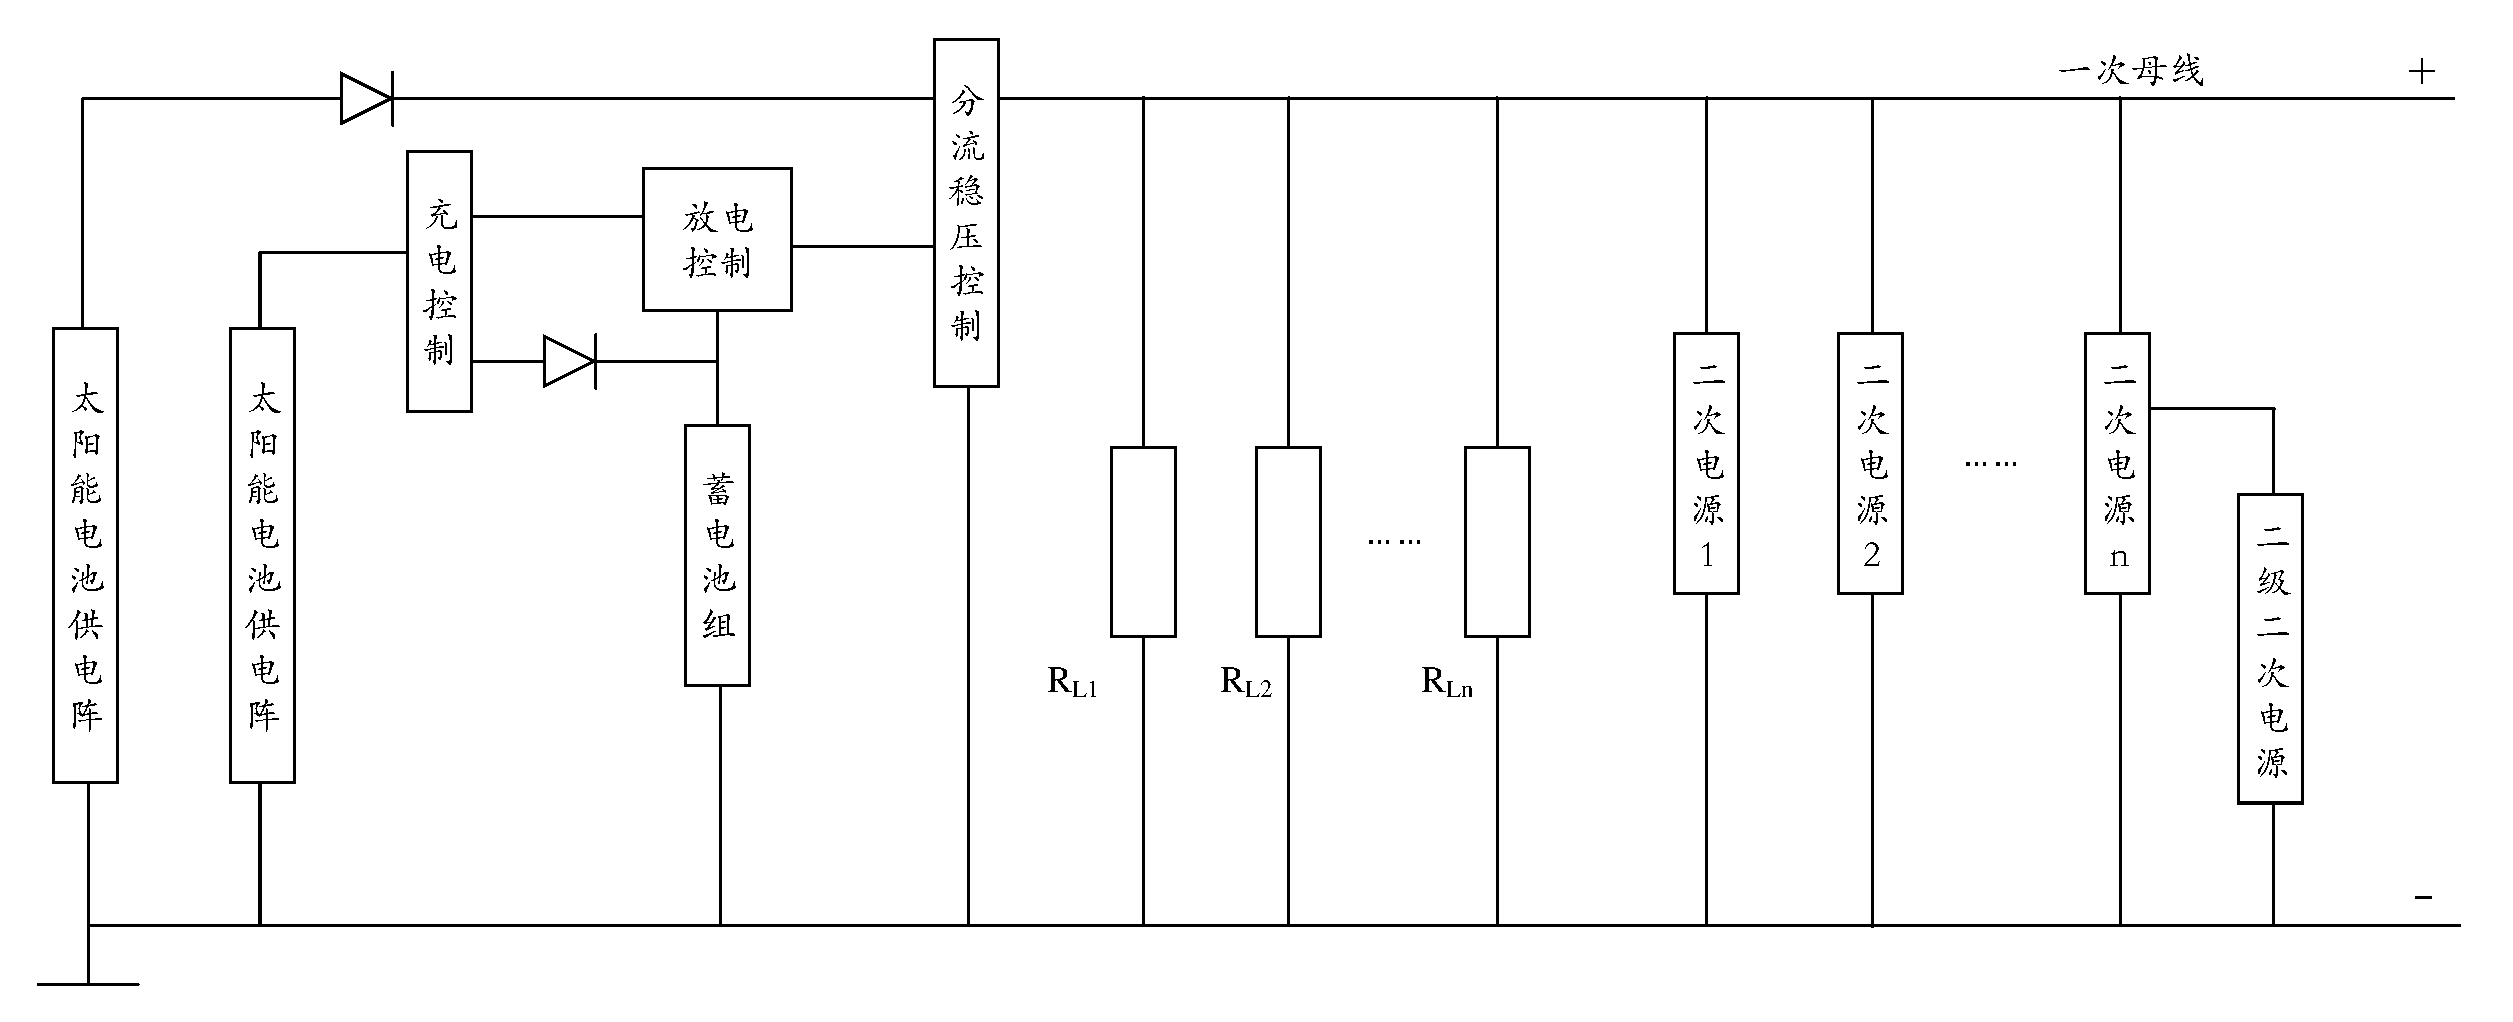
\includegraphics[width=15cm]{chapter1.pdf}\\
   \caption{一种航空航天卫星电源系统结构示意图}\label{fig:chap1:background}
\end{figure}

为确保卫星电源稳定可靠工作,目前国内卫星研制过程中迫切需要针对卫星电源的稳定性展开分析。由于空间卫星电源系统工作在极其特殊的环境中,复杂的空间电源系统受到电磁干扰、温度脉冲以及电子辐射等外界扰动后可能会出现系统性能快速变差的现象,不能稳定可靠地为电子设备提供电源。这种潜在的系统脆弱性特征会对航空航天卫星的安全工作造成重大威胁,因此有必要在卫星设计阶段针对空间电源系统潜在的脆弱性特征进行分析,找出导致系统脆弱性的薄弱环节。针对脆弱性问题,采取措施并进行方案优化。
\section{国内外研究现状}
\label{sec:chap1:situation}
\subsection{脆弱性研究起源}
不同于控制系统稳定性,对于脆弱性现象的研究覆盖多个学科,不同领域对脆弱性现象的研究侧重点不同,至今依然没有一个公认的脆弱性概念。“脆弱性”概念最先在流行病学领域中被提出\cite{Nkhuwa2003Human,Lili2010},描述的是某些地区更容易发生流行病或哪些部位更容易被感染。在~20~世纪~40~年代,White. G. F~在研究世界自然灾害时,提出了人类本身对自然灾害“适应和调整”的观点\cite{GF1945}。这一观点也被认为是脆弱性研究的最初始状态,是还没有形成脆弱性具体概念的萌芽期。从~20~世纪~70~年代起,生物学家们开始研究生物领域的“脆弱性”现象。学者~M. Pacifici~分析研究了气候变化对生态系统中物种多样性带来的脆弱性影响,并建立了三种评估气候脆弱性的模型\cite{Miche2015}。1980~年之后,“脆弱性”概念在全球环境生态变化的研究论文中大量频繁地出现,越来越多的生态及环境科学研究者开始关注生态环境领域内的脆弱性现象。同时,“脆弱性”概念也逐渐在社会学、经济学以及工程学中被人关注。在经济学领域和环境生态学领域从类似风险的角度来分析脆弱性概念,Cutter.S.L~与~Gabor.T~等学者认为脆弱性是对于未知情况的不可预测而产生的可能性或不确定性,是系统受到不利因素或者受到损害的可能性或不确定性\cite{SL1996,TG1979}。社会科学中的学者从应对能力角度来分析脆弱性概念,认为脆弱性是指社会群体及组织暴露在灾害冲击下潜在的受灾因素、受伤害程度以及应对灾害能力的大小。Timmernan. P~与~Tuner.B.L~考虑到外界环境对系统产生的后果,将脆弱性定义为系统受不利影响或损坏的程度\cite{Toronto1981,TN2003},在此之后~Dow.K、Bohle.W.C~等人分别从不同角度在不同领域对“脆弱性”概念进行了诠释\cite{K1992,WC1988}。

最近~20~年内,对于脆弱性概念的研究越来越多元化,各个不同学科领域内对脆弱性的定义与诠释加深了对“脆弱性”概念的理解。近年来,资源与社会经济系统领域的学者将脆弱性概念作为研究热点,引入了测量技术和定量分析模型使得脆弱性研究更加规范化。I.Kelman~利用脆弱性和弹性分析气候变化,减灾风险和可持续发展之间的相通之处,指出气候脆弱性可能导致“多次暴露”的威胁\cite{IK2015}。在经济学领域,脆弱性概念也是近几年的研究热点。基于~2008-2009~年金融危机引发的欧洲经济衰退,Fingleton~等人调查了欧元地区对经济危机的脆弱性和弹性,并通过建立空间面板模型对金融危机进行预测\cite{Fingleton2015}。脆弱性概念已经在各个学科领域引起了重视,各行各业的研究人员都在对自己领域内脆弱的现象开展研究。
%%%%%%%%%%%%%%%%%%%%%%%%%%%%%%%%%%%%%%%%%%%%%%%%%%%%%%%%%%%%%%%%%%%%
\subsection{国内外脆弱性研究现状}
自“脆弱性”概念提出以来,一直用于环境科学、流行病科学以及人文社会科学领域,直到~1990~年以后,脆弱性概念逐渐进入工程领域,1997~年~L.H.Keel~和~S.P.Bhattacharyya~发表了阐述控制系统脆弱性的著名论文~\raisebox{0.5mm}{------}《Robust, Fragile, or Optimal~?》\cite{Keel1997}。这篇论文对由~$H_2$、$H_{\infty}$~以及~$l$~等鲁棒控制器组成的控制系统进行研究,发现这些优化后的闭环控制系统在特定的外部扰动下很容易产生不稳定的状态,系统的幅值裕度和相位裕度都很差。他们采用“脆弱性”概念来描述优化控制系统的这种隐性特性,吸引了许多工程控制领域研究人员对控制系统脆弱特性进行研究。F. Blanchini~与~R. Lo Cigno~等人针对通信领域信号的鲁棒性与脆弱性问题展开研究,建立了用于分析~ATM~网络中单信道信息流脆弱性问题的数学模型,优化了信号噪声的控制算法\cite{Blanchini1998Control}。P.M. Makila~等人对控制系统因系统零极点导致的脆弱性现象进行了研究和分析,并针对~$H_2$~及~$H_{\infty}$~等鲁棒优化控制器在外部扰动作用下产生不稳定的现象进行分析与研究\cite{Makila1999Fragility}。Iury Bessa,Hussama Ismail~以及~Reinaldo Palhares~等人针对数字控制系统的不确定性进行分析并提出了数字系统脆弱性镇定的概念\cite{Bessa2017Formal}。对于控制系统脆弱性的研究主要集中在研究经过优化后的控制系统稳定性变差的现象。由于优化控制器针对所需改进的系统性能参数进行优化处理,容易忽略系统的其他性能参数,即优化后的控制系统可能具有较差的稳定性。许多研究人员将控制系统优化过后稳定性变差的特性定义为系统脆弱性,并研究其具体的产生原因及解决方法。

国内学者从~20~世纪~50~年代开始接触脆弱性概念,在国内脆弱性一词最先出现在计算机网络领域,用于分析与描述节点微小扰动导致计算机网络大规模瘫痪的现象\cite{Dong2003Computerfragile}。随着中国科技的发展,脆弱性概念逐渐在自然灾害、社会系统、生态环境、经济系统以及煤炭石油资源等诸多领域被人提及,中国学者对于脆弱性概念的研究越发频繁。在生态环境领域,乔青、高吉喜等人认为生态脆弱性是在受到外界干扰时,生态环境抵抗能力变弱或受到影响后不容易恢复至原状态的特征,体现为状态易变性和状态难恢复性\cite{QIAO2008}。陶和平等人对生态环境脆弱性理解为生态环境系统对外界干扰的敏感程度以及环境资源向不利于人类利用的方向发展的现象\cite{Tao2006}。在经济学领域,杨爱婷等人认为经济系统脆弱性体现在社会经济容易受到外界环境的干扰或不确定事件的影响,破坏了系统的适应性并损害了系统本身的各项能力\cite{Yang2012}。在电力系统中,白加林与刘天琪等人对电力系统领域中的脆弱性现象定义为因人为干预、信息、计算以及保护控制系统等因素影响而潜伏着大面积停电的危险状态\cite{Bai2008PowerSystemfragile}。电力系统脆弱性研究有助于分析与预防潜在的大面积停电重大事故,已经成为加强电网、预防电力灾变的一项重要分析指标。国内学者对于脆弱性概念接触的相对较晚,大部分学者认为脆弱性是一种系统自身固有的属性,在正常工作状态下并不显现。而当系统受到内部或外部的特定扰动时,系统表现出脆弱性特征。不同系统的脆弱性特征不同,但主要都体现在系统的状态和功能的变化。系统的脆弱性主要是由系统结构所决定的,外界扰动是系统表现出脆弱特性的诱因,因此脆弱性特征最终体现于控制系统对外部摄动的灵敏性以及相应的恢复能力。
\subsection{空间电源研究现状}%稳定性、可靠性、脆弱性
近几年航空航天领域的学者们对空间电源系统的性能尤为关注,李冬辉、高金艳等人对~S3R~架构的卫星电源进行分析与研究,提出了一种优化电路稳健性的设计方法,提高空间电源系统的可靠性\cite{Li2015,Gao2014master}。针对~S3R~架构卫星系统特有的功率调节系统,王乐乐、刘元默等人依据稳定性阻抗判据研究了在大功率脉冲负载作用下,~S3R~架构卫星电源系统的稳定性问题\cite{Wang2014}。对于低轨卫星电源系统,耿卫东、罗顺等人通过研究与优化电源功率分配系统,最大限度地利用太阳电池阵的能源,优化了航天器的设计\cite{Luo2011master}。

航空航天领域中,对于脆弱性的研究集中在卫星系统导航信号及整体卫星系统各环节之间的兼容性。刘春保等人从卫星导航信号的角度入手,分析与研究卫星系统的脆弱性\cite{Liu2015},过低的导航信号功率会使得用户无法较好地获得卫星导航服务,导致卫星导航系统的脆弱性。战兴群、严凯等人对全球导航卫星系统~(GNSS)~进行脆弱性分析\cite{Yan2013},将~GNSS~系统脆弱性分成系统脆弱性、传播脆弱性以及电磁环境脆弱性三类,分析脆弱性形成的机理以及对系统产生的影响。李云志等人从系统的层面分析卫星应用系统的脆弱性\cite{Li2015phd},从技术性及非技术性两个方面构建脆弱性评价体系,并分别分析脆弱性产生的原因以及对系统造成的影响。

航空航天系统结构复杂、影响因素多,关注点不同得到的系统脆弱性的定义就不同。空间电源系统脆弱性的分析主要关注点在于电源系统的稳定性与系统性能,因此本文在航空航天领域恶劣的工作环境背景中,给出空间电源系统脆弱性概念并将其引入控制系统理论中,构建空间电源系统脆弱性分析理论与量化评估数学模型。
\section{待解决的问题}
\label{sec:chap1:Todolist}
对于空间电源这样高可靠系统的脆弱性分析与量化研究依然存在很多待解决的问题,如~:
\begin{enumerate}[(1)]
  \item 脆弱性概念是近几年引入控制系统的概念,对于控制系统的脆弱性描述尚不清晰,特别是脆弱性概念与控制系统稳定性、可靠性以及鲁棒性概念之间的区别与联系尚显模糊;
  \item 控制系统中脆弱性研究主要以研究数学模型为主,实际落实到电源系统的研究和分析相对较少;
  \item 对于控制系统脆弱程度的分析与研究较少,脆弱性量化分析的相关研究未形成严格的理论体系。
 \end{enumerate}
\section{主要研究内容和章节划分}
\label{sec:chap1:content}
本文针对空间电源系统脆弱性分析与量化研究中待解决的问题,从控制系统理论的角度分析了系统稳定性、可靠性、鲁棒性与脆弱性之间的区别与联系,并给出科学的控制系统脆弱性定义。针对空间电源特殊的工作环境,通过查阅文献建立了工作在太空恶劣环境中电子元器件的数学模型。在此基础上,建立了空间电源系统脆弱性分析与量化评估的具体数学模型,以基于~Buck~变换器的空间电源降压系统为例,量化分析系统在电阻、电容、电感元件存在不确定性时的脆弱性并识别出电源系统的薄弱环节。本文的主要研究内容和章节划分为:

第~1~章~:查阅国内外“空间卫星电源”、“脆弱性分析”等相关领域研究文献与论文,对脆弱性概念的起源与发展以及脆弱性在工学领域的研究现状做了详细的调研与综述,为后续研究空间电源系统脆弱性与量化分析方法提供必要的理论依据。在明确研究对象的基础上,科学提炼出待解决的问题,确定研究方法、目标和技术路线;

第~2~章~:针对空间卫星电源系统特殊的工作环境进行分析,将恶劣的太空环境具体化为极端温度环境与极端辐射环境。通过查阅在极端温度和极端辐射实验环境中电子元件参数的变化趋势,结合空间电源特殊的工作环境,建立了空间电源系统中电阻、电容以及电感元件的数学模型;

第~3~章~:从控制系统理论的角度分析了系统稳定性、可靠性、鲁棒性以及脆弱性概念的区别和联系,给出了本文中脆弱性的具体定义。根据脆弱性概念的具体定义,结合控制系统不确定性的数学描述、系统灵敏度以及系统鲁棒稳定的相关概念,采用系统在不同工作环境中鲁棒稳定裕度参数的变化趋势来描述系统脆弱性;

第~4~章~:在第~3~章的基础上,分析不同工作环境下系统鲁棒稳定裕度参数拟合得到的鲁棒稳定裕度曲线。根据系统脆弱性的概念选择鲁棒稳定裕度曲线中能够反映脆弱特征的脆弱性指标,结合多指标融合、权重分配以及综合评价等相关理论,建立了控制系统脆弱性量化评估数学模型;

第~5~章~:以空间电源系统中基于~Buck~变换器的降压电路系统为例,根据第~2~章中建立的电阻、电容、电感模型模拟电源系统在不同工作环境中参数值的变化,分别针对电阻、电容以及电感元件的不确定性进行脆弱性分析与量化评估。借助~MATLAB~软件对基于~Buck~变换器的空间电源系统进行建模,运用~Python~编写脆弱性量化评估算法,量化分析系统的脆弱性并识别导致系统脆弱的薄弱环节;

第~6~章~:总结本文的研究工作,对本文中控制系统脆弱性量化数学模型的优点和不足进行了详细的阐述,并为后续研究工作提出了若干点建议与展望。

\bigskip
通过以上~6~章研究工作,完成了空间电源系统脆弱性分析与量化评估的理论研究及实验验证与分析,具体技术路线如图~\ref{fig:chap1:step}~所示。
%%%%%%%%%%%%%%%%%%%%%%%%%%%%%%%%%%%%%%%%%%%%%%%%%%%%%%%%%%%%%%%%
\begin{figure}[hbp]
  \centering
  % Requires \usepackage{graphicx}
  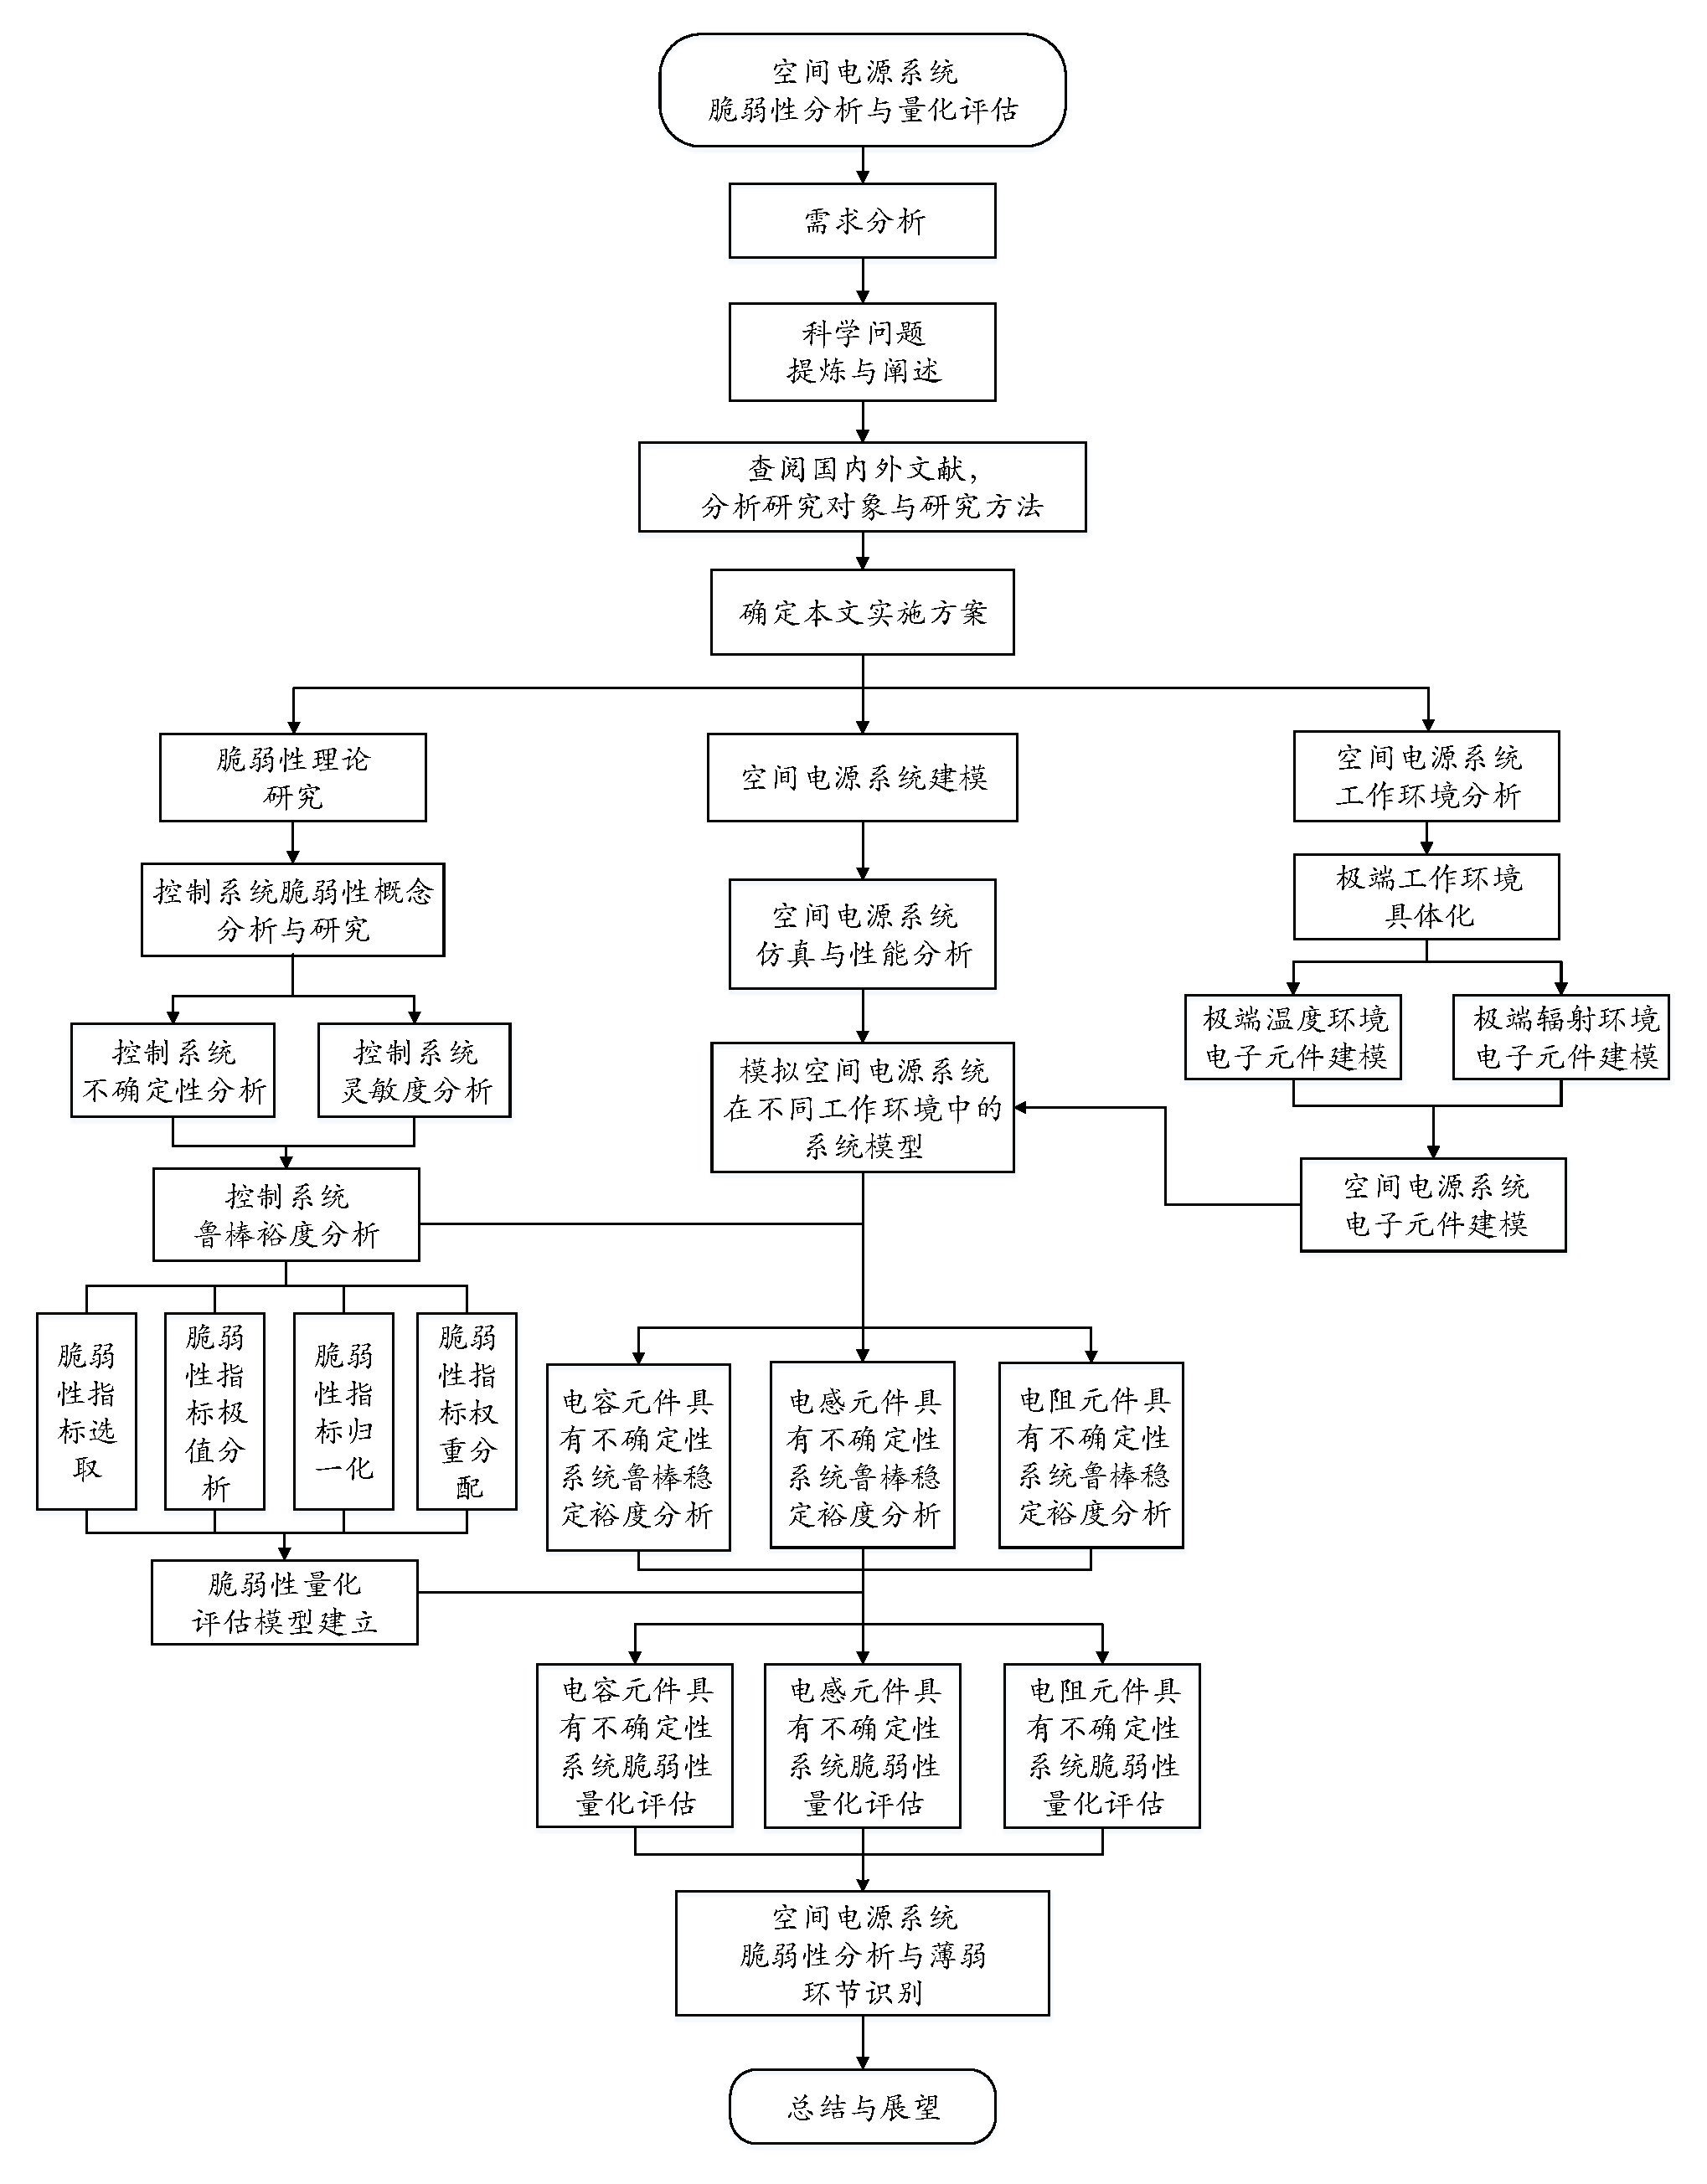
\includegraphics[width=16cm]{Technical_Route.pdf}\\
  \caption{技术路线图}\label{fig:chap1:step}
\end{figure}
